\documentclass[a4paper,12pt,oneside,openany]{memoir}

%%% Задаем поля, отступы и межстрочный интервал %%%

\usepackage[left=30mm, right=15mm, top=20mm, bottom=20mm]{geometry} % Пакет geometry с аргументами для определения полей
\pagestyle{plain} % Убираем стандарные для данного класса верхние колонтитулы с заголовком текущей главы, оставляем только номер страницы снизу по центру
\parindent=1.25cm % Абзацный отступ 1.25 см, приблизительно равно пяти знакам, как по ГОСТ
\usepackage{indentfirst} % Добавляем отступ к первому абзацу
%\linespread{1.3} % Межстрочный интервал (наиболее близко к вордовскому полуторному) - тут вместо этого используется команда OnehalfSpacing*

%%% Задаем языковые параметры и шрифт %%%

\usepackage[english, russian]{babel}                % Настройки для русского языка как основного в тексте
\babelfont{rm}{Times New Roman}                     % TMR в качестве базового roman-щрифта

%%% Задаем стиль заголовков и подзаголовков в тексте %%%

\setsecnumdepth{subsection} % Номера разделов считать до третьего уровня включительно, т.е. нумеруются только главы, секции, подсекции
\renewcommand*{\chapterheadstart}{} % Переопределяем команду, задающую отступ над заголовком, чтобы отступа не было
\renewcommand*{\printchaptername}{} % Переопределяем команду, печатающую слово "Глава", чтобы оно не печалось
%\renewcommand*{\printchapternum}{} % То же самое для номера главы - тут не надо, номер главы оставляем
\renewcommand*{\chapnumfont}{\normalfont\bfseries} % Меняем стиль шрифта для номера главы: нормальный размер, полужирный
\renewcommand*{\afterchapternum}{\hspace{1em}} % Меняем разделитель между номером главы и названием
\renewcommand*{\printchaptertitle}{\normalfont\bfseries\centering\MakeUppercase} % Меняем стиль написания для заголовка главы: нормальный размер, полужирный, центрированный, заглавными буквами
\setbeforesecskip{20pt} % Задаем отступ перед заголовком секции
\setaftersecskip{20pt} % Ставим такой же отступ после заголовка секции
\setsecheadstyle{\raggedright\normalfont\bfseries} % Меняем стиль написания для заголовка секции: выравнивание по правому краю без переносов, нормальный размер, полужирный
\setbeforesubsecskip{20pt} % Задаем отступ перед заголовком подсекции
\setaftersubsecskip{20pt} % Ставим такой же отступ после заголовка подсекции
\setsubsecheadstyle{\raggedright\normalfont\bfseries}  % Меняем стиль написания для заголовка подсекции: выравнивание по правому краю без переносов, нормальный размер, полужирный

%%% Задаем параметры оглавления %%%

\addto\captionsrussian{\renewcommand\contentsname{Содержание}} % Меняем слово "Оглавление" на "Содержание"
\setrmarg{2.55em plus1fil} % Запрещаем переносы слов в оглавлении
%\setlength{\cftbeforechapterskip}{0pt} % Эта команда убирает интервал между заголовками глав - тут не надо, так красивее смотрится
\renewcommand{\aftertoctitle}{\afterchaptertitle \vspace{-\cftbeforechapterskip}} % Делаем отступ между словом "Содержание" и первой строкой таким же, как у заголовков глав
%\renewcommand*{\chapternumberline}[1]{} % Делаем так, чтобы номер главы не печатался - тут не надо
\renewcommand*{\cftchapternumwidth}{1.5em} % Ставим подходящий по размеру разделитель между номером главы и самим заголовком
\renewcommand*{\cftchapterfont}{\normalfont\MakeUppercase} % Названия глав обычным шрифтом заглавными буквами
\renewcommand*{\cftchapterpagefont}{\normalfont} % Номера страниц обычным шрифтом
\renewcommand*{\cftchapterdotsep}{\cftdotsep} % Делаем точки до номера страницы после названий глав
\renewcommand*{\cftdotsep}{1} % Задаем расстояние между точками
\renewcommand*{\cftchapterleader}{\cftdotfill{\cftchapterdotsep}} % Делаем точки стандартной формы (по умолчанию они "жирные")
\maxtocdepth{subsection} % В оглавление попадают только разделы первыхтрех уровней: главы, секции и подсекции

%%% Выравнивание и переносы %%%

%% http://tex.stackexchange.com/questions/241343/what-is-the-meaning-of-fussy-sloppy-emergencystretch-tolerance-hbadness
%% http://www.latex-community.org/forum/viewtopic.php?p=70342#p70342
\tolerance 1414
\hbadness 1414
\emergencystretch 1.5em                             % В случае проблем регулировать в первую очередь
\hfuzz 0.3pt
\vfuzz \hfuzz
%\dbottom
%\sloppy                                            % Избавляемся от переполнений
\clubpenalty=10000                                  % Запрещаем разрыв страницы после первой строки абзаца
\widowpenalty=10000                                 % Запрещаем разрыв страницы после последней строки абзаца
\brokenpenalty=4991                                 % Ограничение на разрыв страницы, если строка заканчивается переносом

%%% Объясняем компилятору, какие буквы русского алфавита можно использовать в перечислениях (подрисунках и нумерованных списках) %%%
%%% По ГОСТ нельзя использовать буквы ё, з, й, о, ч, ь, ы, ъ %%%
%%% Здесь также переопределены заглавные буквы, хотя в принципе они в документе не используются %%%

\makeatletter
    \def\russian@Alph#1{\ifcase#1\or
       А\or Б\or В\or Г\or Д\or Е\or Ж\or
       И\or К\or Л\or М\or Н\or
       П\or Р\or С\or Т\or У\or Ф\or Х\or
       Ц\or Ш\or Щ\or Э\or Ю\or Я\else\xpg@ill@value{#1}{russian@Alph}\fi}
    \def\russian@alph#1{\ifcase#1\or
       а\or б\or в\or г\or д\or е\or ж\or
       и\or к\or л\or м\or н\or
       п\or р\or с\or т\or у\or ф\or х\or
       ц\or ш\or щ\or э\or ю\or я\else\xpg@ill@value{#1}{russian@alph}\fi}
\makeatother

%%% Задаем параметры оформления рисунков и таблиц %%%

\usepackage{graphicx, caption, subcaption} % Подгружаем пакеты для работы с графикой и настройки подписей
\graphicspath{{images/}} % Определяем папку с рисунками
\captionsetup[figure]{font=small, width=\textwidth, name=Рисунок, justification=centering} % Задаем параметры подписей к рисункам: маленький шрифт (в данном случае 12pt), ширина равна ширине текста, полнотекстовая надпись "Рисунок", выравнивание по центру
\captionsetup[subfigure]{font=small} % Индексы подрисунков а), б) и так далее тоже шрифтом 12pt (по умолчанию делает еще меньше)
\captionsetup[table]{singlelinecheck=false,font=small,width=\textwidth,justification=justified} % Задаем параметры подписей к таблицам: запрещаем переносы, маленький шрифт (в данном случае 12pt), ширина равна ширине текста, выравнивание по ширине
\captiondelim{ --- } % Разделителем между номером рисунка/таблицы и текстом в подписи является длинное тире
\setkeys{Gin}{width=\textwidth} % По умолчанию размер всех добавляемых рисунков будет подгоняться под ширину текста
\renewcommand{\thesubfigure}{\asbuk{subfigure}} % Нумерация подрисунков строчными буквами кириллицы
%\setlength{\abovecaptionskip}{0pt} % Отбивка над подписью - тут не меняем
%\setlength{\belowcaptionskip}{0pt} % Отбивка под подписью - тут не меняем
\usepackage[section]{placeins} % Объекты типа float (рисунки/таблицы) не вылезают за границы секциии, в которой они объявлены

%%% Задаем параметры ссылок и гиперссылок %%% 

\usepackage{hyperref}                               % Подгружаем нужный пакет
\hypersetup{
    colorlinks=true,                                % Все ссылки и гиперссылки цветные
    linktoc=all,                                    % В оглавлении ссылки подключатся для всех отображаемых уровней
    linktocpage=true,                               % Ссылка - только номер страницы, а не весь заголовок (так выглядит аккуратнее)
    linkcolor=red,                                  % Цвет ссылок и гиперссылок - красный
    citecolor=red                                   % Цвет цитировний - красный
}

%%% Настраиваем отображение списков %%%

\usepackage{enumitem}                               % Подгружаем пакет для гибкой настройки списков
\renewcommand*{\labelitemi}{\normalfont{--}}        % В ненумерованных списках для пунктов используем короткое тире
\makeatletter
    \AddEnumerateCounter{\asbuk}{\russian@alph}     % Объясняем пакету enumitem, как использовать asbuk
\makeatother
\renewcommand{\labelenumii}{\asbuk{enumii})}        % Кириллица для второго уровня нумерации
\renewcommand{\labelenumiii}{\arabic{enumiii})}     % Арабские цифры для третьего уровня нумерации
\setlist{noitemsep, leftmargin=*}                   % Убираем интервалы между пунками одного уровня в списке
\setlist[1]{labelindent=\parindent}                 % Отступ у пунктов списка равен абзацному отступу
\setlist[2]{leftmargin=\parindent}                  % Плюс еще один такой же отступ для следующего уровня
\setlist[3]{leftmargin=\parindent}                  % И еще один для третьего уровня

%%% Счетчики для нумерации объектов %%%

\counterwithout{figure}{chapter}                    % Сквозная нумерация рисунков по документу
\counterwithout{equation}{chapter}                  % Сквозная нумерация математических выражений по документу
\counterwithout{table}{chapter}                     % Сквозная нумерация таблиц по документу

%%% Реализация библиографии пакетами biblatex и biblatex-gost с использованием движка biber %%%

\usepackage{csquotes} % Пакет для оформления сложных блоков цитирования (biblatex рекомендует его подключать)
\usepackage[%
backend=biber,                                      % Движок
bibencoding=utf8,                                   % Кодировка bib-файла
sorting=none,                                       % Настройка сортировки списка литературы
style=gost-numeric,                                 % Стиль цитирования и библиографии по ГОСТ
language=auto,                                      % Язык для каждой библиографической записи задается отдельно
autolang=other,                                     % Поддержка многоязычной библиографии
sortcites=true,                                     % Если в квадратных скобках несколько ссылок, то отображаться будут отсортированно
movenames=false,                                    % Не перемещать имена, они всегда в начале библиографической записи
maxnames=5,                                         % Максимальное отображаемое число авторов
minnames=3,                                         % До скольки сокращать число авторов, если их больше максимума
doi=false,                                          % Не отображать ссылки на DOI
isbn=false,                                         % Не показывать ISBN, ISSN, ISRN
]{biblatex}[2016/09/17]
\DeclareDelimFormat{bibinitdelim}{}                 % Убираем пробел между инициалами (Иванов И.И. вместо Иванов И. И.)
\addbibresource{biba.bib}                           % Определяем файл с библиографией

%%% Скрипт, который автоматически подбирает язык (и, следовательно, формат) для каждой библиографической записи %%%
%%% Если в названии работы есть кириллица - меняем значение поля langid на russian %%%
%%% Все оставшиеся пустые места в поле langid заменяем на english %%%

\DeclareSourcemap{
  \maps[datatype=bibtex]{
    \map{
        \step[fieldsource=title, match=\regexp{^\P{Cyrillic}*\p{Cyrillic}.*}, final]
        \step[fieldset=langid, fieldvalue={russian}]
    }
    \map{
        \step[fieldset=langid, fieldvalue={english}]
    }
  }
}

%%% Прочие пакеты для расширения функционала %%%

\usepackage{longtable,ltcaption}                    % Длинные таблицы
\usepackage{multirow,makecell}                      % Улучшенное форматирование таблиц
\usepackage{booktabs}                               % Еще один пакет для красивых таблиц
\usepackage{soulutf8}                               % Поддержка переносоустойчивых подчёркиваний и зачёркиваний
\usepackage{icomma}                                 % Запятая в десятичных дробях
\usepackage{hyphenat}                               % Для красивых переносов
\usepackage{textcomp}                               % Поддержка "сложных" печатных символов типа значков иены, копирайта и т.д.
\usepackage[version=4]{mhchem}                      % Красивые химические уравнения
\usepackage{amsmath}                                % Усовершенствование отображения математических выражений 
\usepackage{dsfont}
\usepackage{bm}

%%% Вставляем по очереди все содержательные части документа %%%

\begin{document}

\thispagestyle{empty}

\begin{center}
    МИНИСТЕРСТВО НАУКИ И ВЫСШЕГО ОБРАЗОВАНИЯ \\ РОССИЙСКОЙ ФЕДЕРАЦИИ

    \vspace{20pt}
    
    Федеральное государственное автономное \\ образовательное учреждение высшего образования \\
    "<Московский физико-технический институт (национальный исследовательский университет)"> \\

    \vspace{20pt}

	Физтех-школа Радиотехники и Компьютерных Технологий
\end{center}

\vfill

\begin{center}
    РЕФЕРАТ \\  
    по дисциплине \\
    \textit{"<Защита информации">}

    \vspace{20pt}

    по теме: \\
    \uppercase{Задачи, лежащие в основе постквантовых KEM}
\end{center}

\vfill

    \noindent Студент: \\
    \textit{Группа № Б01-108 \hfill А.Л. Симанкович}

\vspace{20pt}

\begin{center}
    Долгопрудный 2024
\end{center}                                     % Титульник

\newpage % Переходим на новую страницу
\setcounter{page}{2} % Начинаем считать номера страниц со второй
\OnehalfSpacing* % Задаем полуторный интервал текста (в титульнике одинарный, поэтому команда стоит после него)

\tableofcontents*                                   % Автособираемое оглавление

\chapter{Введение}
\label{ch:intro}

\section{Актуальность проблемы}
Ассиметричное шифрование (шифрование с открытым ключом) лежит в основе множества ключевых сетевых протоколов (TLS, SSH, HTTPS). Однако устойчивость используемых в данный момент алгоритмов шифрования находится под угрозой квантовых компьютеров. При создании достаточно большого (в терминах количества кубитов -- квантовых битов) компьютера, уже разработанные квантовые алгоритмы позволят получить доступ к огромному массиву информации, передающейся по сети. Под угрозой находятся переписки, банковские транзакции, личные данные, системы удаленного управления и т.п.

Для защиты от атак с помощью квантовых компьютеров разрабатываются специальные -- постквантовые алгоритмы. Основным отличием от классических алгоритмов они отличаются требованием устойчивости как к классическим, так и квантовым атакам. При этом шифрование должно производится на классических компьютерах. Это позволит внедрить алгоритмы заранее и использовать повсеместно.

Стратегия "Harvest now, decrypt later"\; заключается в сборе открытых ключей и зашифрованных данных сейчас, с расчетом на появление технологий, позволяющих расшифровать их в будущем. Это позволит злоумышленникам воспользоваться слабостью нынешнего шифрования. Взлом этих алгоритмов также позволит подменить подписи, использованные в прошлом, переписав историю транзакций (например, в блокчейне). Поэтому разработка и внедрение постквантовых алгоритмов должно производится задолго до того, как появятся квантовые компьютеры, представляющие угрозу (Y2Q или Q-day).

\section{Механизмы шифрования ключа (KEM)}

Задачи создания защищенного канала решаются наиболее быстро и удобно с помощью симметричного шифрования. В этом случае обе стороны используют общий секретный ключ. Недостаток этого подхода заключается в необходимости доставить секретный ключ, не раскрыв его злоумышленникам. В случае обеспечения такого доступа между агентами по сети этот недостаток становится критическим. Для его исправления используются KEM (Key Encapsulation Mechanism -- механизм шифрования ключа).

KEM основаны на ассиметричном шифровании с открытым ключом. Агент A генерирует асимметричную пару ключей $(s, p)$, открытый ключ $p$ отправляет по сети агенту B. Агент B генерирует симметричный секретный ключ $k$, шифрует его с помощью открытого ключа $p$ и отправляет шифр $c$. Агент A дешифрует $c$ с помощью $s$, получая симметричный ключ $k$.

\section{Классические алгоритмы}

Все алгоритмы с открытым ключом опираются на сложность инвертирования некоторой односторонней функции. Такая функция должна иметь полиномиальную сложность при вычислении и экспоненциальную сложность при инвертировании. В прикладном смысле это означает, что шифрование с помощью открытого ключа должно быть быстрым, а дешифровка быстрой только с помощью секретного ключа.

На данный момент самые широкораспространенные алгоритмы используют факторизацию целых чисел (например, RSA), дискретный логарифм (EdDSA). Все эти задачи уязвимы к алгоритму Шора -- квантовому алгоритму, который использует квантовое преобразование Фурье (QFT).

\section{Постквантовые алгоритмы}

Постквантовые алгоритмы основаны на задачах из различных областей математики, включая:
\begin{itemize}
	\item Решетки (Lattice-based);
	\item Хэши (Hash-based);
	\item Коды ошибок (Code-based);
	\item Изогении (Isogeny-based).
\end{itemize}

Мы рассмотрим принципы работы нескольких из них.

\endinput                                     % Введение
\chapter{Алгоритмы на решетках}
\label{ch:chap2}

В этой главе будут задачи SVP/SIS и LWE, и основанные на них алгоритмы шифрования.

\section{Решетки как математическая структура}
\label{sec:lattice_math}

Решетка -- это периодическая ``сетка'' в пространстве $Z^m$.
Для каждой решетки можно выбрать базис, причем он не единственный.

\begin{figure}[ht]
	\centering
	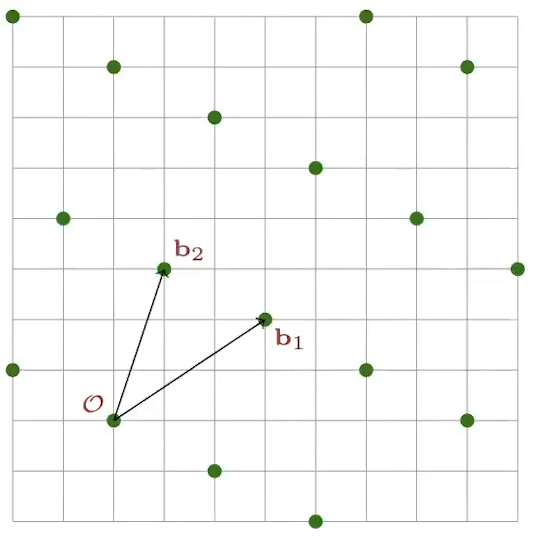
\includegraphics[width=0.5\textwidth]{lattice_basis}
	\caption{Пример решетки и ее базиса при $m = 2$}
	\label{fig:lattice_basis}
\end{figure}

Для них существует некоторый набор ``стандартных'', хорошо изученных задач. Например, GapSVP, SIVP (Shortest Independent Vectors Problem). Эти задачи в сложных случаях (для сложных наборов параметров) не имеют полиномиальных алгоритмов решения.

\section{SVP (Shortest Vector Problem)}

Постановка задачи проста: найти самый короткий вектор $\bm{b_0}$ в решетке $\mathcal{L}$, заданной каким-то базисом.

Сложность задачи растет с размерностью решетки $m$. Обычно рассматриваются приближенные задачи -- поиск вектора с длиной меньше $\gamma \boldsymbol{b_0}$. Имеющиеся алгоритмы (в том числе квантовые) требуют экспоненциальных памяти и времени для задачи с $\gamma = poly(m)$ \cite{svp}.

Квантовые алгоритмы не исправляют ситуацию, поскольку не говорят ничего о геометрических свойствах. Например, алгоритм Шора хорошо справляется с поиском групповой структуры, но не позволяет находить кратчайшие вектора в геометрическом смысле.

\section{SIS (Short Integer Solution)}

Эта задача является алгебраической и на первый взгляд не имеет ничего общего с решетками.

Пусть $\mathds{Z}^n_q$ -- поле векторов размерности $n$ по модулю $q$.
Выберем равномерно случайную матрицу $A \in \mathds{Z}^{n \times m}_q$. Задача -- найти ненулевой $\boldsymbol{z} \in \mathds{Z}^m$ такой, что $A \boldsymbol{z} = \boldsymbol{0} \in \mathds{Z}^n_q$ при условии $\|\boldsymbol{z}\| < \beta \ll q$. 

Если предположить, что SIS сложно решить, то, взяв $m > n \log_2 q$ определим хэш-функцию $f_A: \{0,1\}^m \rightarrow \mathds{Z}^n_q$ как $f_A(\boldsymbol{x}) = A\boldsymbol{x}$. Такая функция будет устойчива к поиску коллизий, поскольку $A\boldsymbol{x} = A \boldsymbol{x'} \Rightarrow A(\boldsymbol{x} - \boldsymbol{x'}) = 0$, то есть $\boldsymbol{z} = \boldsymbol{x} - \boldsymbol{x'} \in \{0, \pm 1\}^m$ -- решение SIS.

\section{Связь SIS и SVP}

Выясним, какое отношение SIS имеет к решеткам.

Матрица $A \in \mathds{Z}^{n \times m}_q$ задает решетку $\mathcal{L^{\perp}} (A) = \{\boldsymbol{z} \in \mathds{Z}^m : A\boldsymbol{z} = \boldsymbol{0}\}$. На Рисунке \ref{fig:lattice_matrix} изображена решетка для случая $m = 2$. Тогда нахождение $\boldsymbol{z}$ для SIS эквивалентно поиску ``короткого'' вектора в решетке $\mathcal{L^{\perp}}(A)$. То есть SIS эквивалентна SVP.

\begin{figure}[ht]
	\centering
	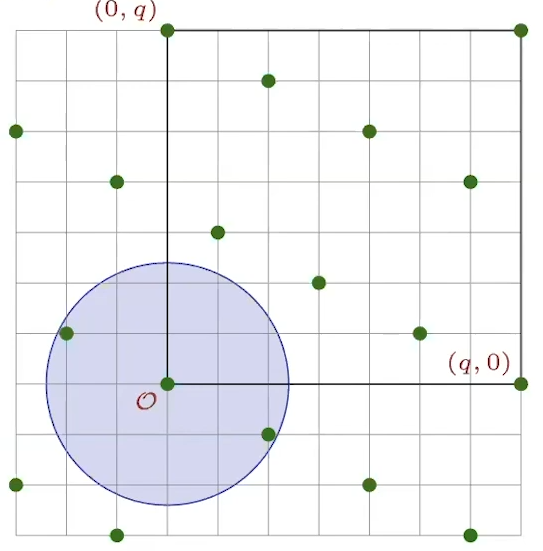
\includegraphics[width=0.5\textwidth]{lattice_matrix}
	\caption{Решетка и ограничение на длину вектора $\boldsymbol{z}$}
	\label{fig:lattice_matrix}
\end{figure}

Важным теоретическим результатом является сведение worst-case (нахождение решения на самых сложных вариантах) к average-case (нахождение решения для случайных вариантов):
Алгоритмом для нахождения ``короткого'' вектора для равномерно случайной $A$ можно решить любую задачу GapSVP и SIVP \cite{Ajtai96}. Поскольку лучшие алгоритмы, которые были найдены, для сложных случаев GapSVP и SIVP -- экспоненциальные, то считается, что полиномиального алгоритма для SIS не существует.

\section{Применение SIS в криптографии}

Предположим, что мы можем сгенерировать равномерно случайную матрицу $A$ с ``секретным ключом'' $T$ (trapdoor). Такой алгоритм существует, почти любая матрица может из равномерного распределения может быть создана в паре с ключом $T$ \cite{short_basis_trapdoor}.
Для подписи мы считаем хэш сообщения $H(\mu)$ и с помощью $T$ находим достаточно короткий $\boldsymbol{z}: A \boldsymbol{z} = H(\mu) \in \mathds{Z}^n_q$.
В качестве $H(\mu)$ можно использовать любую достаточно надежную хэш-функцию (например, SHA).
Для того, чтобы исключить ``обучение'' на выдаваемых $\boldsymbol{z}$ мы будем брать их из дискретного гауссова распределения. Иначе, $T$ может быть восстановлен по набору $\boldsymbol{z}$ для различных $H(\mu)$ \cite{DN12}.

Для создания подписи на другое сообщение $\mu^*$ злоумышленнику требуется найти ``достаточно короткий'' $\boldsymbol{z}$ такой, что $A \boldsymbol{z^*} = H(\mu^*)$. Эта задача и есть SIS.

\section{LWE (Learning With Errors)}

Постановка задачи LWE: необходимо найти секретный $\boldsymbol{s} \in \mathds{Z}^n_q$, зная $\boldsymbol{b}^T = \bm{s}^T A + \bm{e}^T$ -- скалярные произведения случайных векторов с $\boldsymbol{s}$ с некоторой гауссовой ошибкой $\bm{e}$.

Матрица $A$ вновь задает решетку, но уже иначе: $\mathcal{L}(A) = \{ \boldsymbol{z}^T : \boldsymbol{z}^T = \boldsymbol{s}^T A \mod q\}$. Пример приведен на Рисунке \ref{fig:lattice_lwe}. Таким образом, LWE сводится к задаче поиска узла решетки по точке в его окрестности.

\begin{figure}[ht]
	\centering
	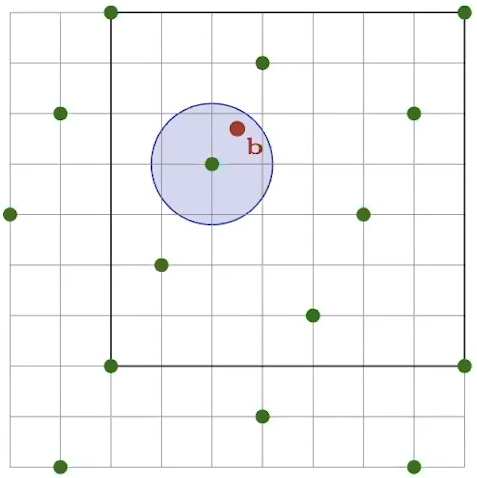
\includegraphics[width=0.5\textwidth]{lattice_lwe}
	\caption{Нахождение узла решетки по точке вблизи него (тут $\bm{e} \notin \mathds{Z}^n_q$ для наглядности)}
	\label{fig:lattice_lwe}
\end{figure}

Теория говорит, что search-LWE -- сложная задача. Есть сведение алгоритма для average-case LWE к worst-case задачам на решетках (GapSVP, SIVP) \cite{Regev05}. Эти задачи считаются не имеющими полиномиального решения даже квантовыми компьютерами, поэтому LWE считается квантово устойчивой.

Более того, можно показать, что если существует алгоритм, отличающий полностью случайные пары $(A, \boldsymbol{b})$ от тех, которые являются скалярным произведением с $\boldsymbol{s}$ (decision-LWE), то его можно свести к алгоритму для search-LWE \cite{Regev05}.

\section{Применение LWE в криптографии}

Агенты А и Б выбирают равномерно случайную матрицу $A \in \mathds{Z}^{n \times n}_q$. Эта матрица будет частью открытого ключа, общего для агентов. После чего агент А выбирает ``короткий'', равномерно случайный вектор $\boldsymbol{s} \in \mathds{Z}^n_q$, Б -- вектор $\boldsymbol{r}$ с такими же свойствами. Агент А вычисляет $\bm{u}^T \approx \bm{r}^T A \in \mathds{Z}^n_q$, агент Б в свою очередь $\bm{v} \approx A \bm{s} \in \mathds{Z}^n_q$. При вычислении $\bm{u}$ и $\bm{v}$ вносится ошибка из гауссова распределения, которое также является заранее выбранным и общеизвестным.

Заметим, что агент А может получить $\bm{r}^T \bm{v} \approx \bm{r}^T A \bm{s} \approx k$. В свою очередь агент Б получает $\bm{u}^T \bm{s} \approx \bm{r}^T A \bm{s} \approx k$. То есть А и Б получили два числа, очень близких к общему числу $k \in \mathds{Z}_q$.

Тогда агент Б может закодировать бит как $c = k + \text{bit} \cdot \frac{q}{2}$.

При дешифровке агент А получает

\begin{equation*}
	c - k \approx \text{bit} \cdot \frac{q}{2} =
	\begin{cases}
		\text{число, близкое к нулю, bit = 0};\\
		\text{число, близкое к } \frac{q}{2} \text{, bit = 1}.
	\end{cases}
\end{equation*}

Для каждого нового бита нужно генерировать новую пару $\bm{s}$, $\bm{r}$, однако существуют способы ослабить это требование.

Рассмотрим задачу со стороны злоумышленника. Он имеет доступ к $\{A, \bm{u}, \bm{v}, c \}$. Его задача -- распознать, $c = k$ или $c = k + \frac{q}{2}$. По сути это -- задача decision-LWE. То есть она считается квантово устойчивой на сегодняшний день. Для злоумышленника набор $\{A, \bm{u}, \bm{v}, c \}$ неотличим от равномерно случайного.

Может показаться, что значения $\bm{r}$ и $\bm{s}$ можно получить обращением матрицы $A$. Однако, попытка применить $A^{-1}$ к $\bm{u}$ или $\bm{v}$ дает
\begin{equation*}
	A^{-1} \bm{u} = A^{-1} A \bm{r} + A^{-1} \bm{e}= \bm{r} + A^{-1} \bm{e}.
\end{equation*}
При этом $A^{-1} \bm{e}$ вносит настолько сильный вклад, что выделить $\bm{r}$ становится невозможным.

\section{Преимущества}

Алгоритмы, основанные на решетках, обладают рядом преимуществ:
\begin{itemize}
	\item задачи на решетках опираются на геометрические свойства, вычисление которых хорошо сопротивляются квантовым атакам;
	\item существуют теоремы, доказывающие, что из worst-case hardness задач следует их average-case hardness;
	\item обладают высокой степенью вычислительного параллелизма за счет линейной структуры.
\end{itemize}

Кроме того, их можно использовать для полностью гомоморфного шифрования (Fully Homomorphic Encryption) -- шифрование, позволяющие совершать математические операции над данными не расшифровывая их.

\endinput                                     % Первая глава
\chapter{Алгоритм на изогениях}
\label{ch:isogenies}

В этой главе будет рассмотрен принцип работы алгоритма SIDH (Supersingular Isogeny Diffie-Hellman).

\section{Изогении как математическая структура}

\subsection{Эллиптические кривые}

Изогении основаны на эллиптических кривых.

Нам понадобится сложение точек на эллиптических кривых (пример на Рисунке \ref{fig:elliptic_curve}) и определение порядка точки: $\deg P = n$, если $[n]P = \mathcal{O}$, где $[n]P$ -- сложение $P$ с самим собой $n$ раз, $\mathcal{O}$ -- нейтральный элемент .

\begin{figure}[ht]
	\centering
	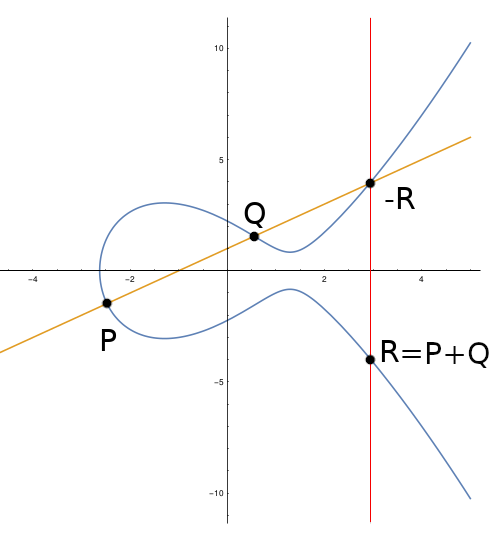
\includegraphics[width=0.5\textwidth]{elliptic_curve}
	\caption{Пример эллиптической кривой}
	\label{fig:elliptic_curve}
\end{figure}

Пусть дана $P \in E$, а точка $S$ вычисляется как $S = [n] P \in E$. 
Классическая задача (используемая в EdDSA) -- дискретный логарифм на эллиптических кривых, ставится так: найти $n$ такое, что $S = [n] P$.

Эта задача сложная для классических компьютеров, но не для квантовых.

\subsection{Изоморфизмы и $j$-инварианты}

С этого момента будем работать в поле $\mathds{F}_{q^2}.$

Для эллиптической кривой $E_a$ можно ввести понятие $j$-инварианта -- специальное число, описывающее данную кривую. Например, для кривой $E_a: y^2 = x^3 + ax^2 + x$ $j$-инвариант задается как $j(E_a) = \frac{256(a^3-3)^3}{a^2-4}$.

Кривые $E$ и $E'$ называются изоморфными ($E \cong E'$), если у них одинаковые $j$-инварианты. Между любыми изоморфными кривыми существует линейное преобразование $\psi$, переводящее одну кривую в другую. Соответственно, существует и обратное ему $\psi^{-1}$:

\begin{equation*}
	\begin{aligned}
		& \psi      &: E \rightarrow E', \qquad & (x, y) \rightarrow (\alpha x + \beta, \gamma y), \\
		& \psi^{-1} &: E' \rightarrow E, \qquad & (x, y) \rightarrow (\alpha' x + \beta', \gamma' y).
	\end{aligned}
\end{equation*}

Заметим, что у них отсутствуют особые точки, то есть $\ker \psi = \{ \mathcal{O}_E \}$, $\ker \psi = \{ \mathcal{O}_E' \}$, где $\mathcal{O}$ -- нейтральный элемент группы.

\subsection{Изогении}

В случае, когда $j$-инварианты не равны, мы можем строить нелинейные отображения. Для некоторых пар $E$, $E'$ у отображений появляются нули в знаменателе. У этих отображений $\ker \varphi$ нетривиален. Тогда $E$ и $E'$ называются изогенными друг другу, а отображение $\varphi$ называется изогенией.

Для любого конечного подмножества $G$ точек на $E$ существует единственная изогения $\varphi$, для которой $\ker \varphi = G$. Формулы Велу (Vélu's formulas) по $G$ вычисляют $\varphi$ и $E'$ \cite{velu_elliptic}.

Композиция изогений сохраняет групповые свойства:
\begin{equation*}
	\varphi(P + Q) = \varphi(P) + \varphi(Q).
\end{equation*}
Размер ядра $\varphi$ будем называть его степенью: $\deg \varphi = \# (\ker \varphi)$. Для композиции изогений существует свойство:
\begin{equation*}
	\deg (\varphi_1 \circ \varphi_2) = \deg(\varphi_1) \cdot \deg(\varphi_2).
\end{equation*}

Таким образом, мы можем строить изогении очень высокого порядка как цепочку композиций изогений малого порядка.

\subsection{Упрощаем начальные условия}

1) Для всех изогений, полученных по формулам Велу выполняется свойство:
\begin{equation*}
	(x, y) \rightarrow (f(x),\; cyf'(x)), \quad c = \text{const}.
\end{equation*}
Поэтому мы можем опускать $y$ в дальнейших выкладках.

2) Для алгоритма требуются изогении порядков $n = 2$ и $n = 3$.

\section{Операции агентов}

Операции агентов достаточно сложны и требуют выкладок в области теории групп. Общая идея заключается в разложении изогении высокого порядка на многократную композицию изогений малых порядков \cite{isogenies}.

\section{Граф $j$-инвариантов}

Для любого простого числа $p$ в поле $\mathds{F}_{p^2}$ существует около $p/12$ особых эллиптических кривых (с точностью до гомоморфизма), которые позволяют ввести на них группу относительно умножения. Каждой из них соответствуют значение $j$-инварианта. На Рисунке \ref{fig:isogenies} приведен пример для $p = 431$ \cite{isogenies}.

\begin{figure}[ht]
	\centering
	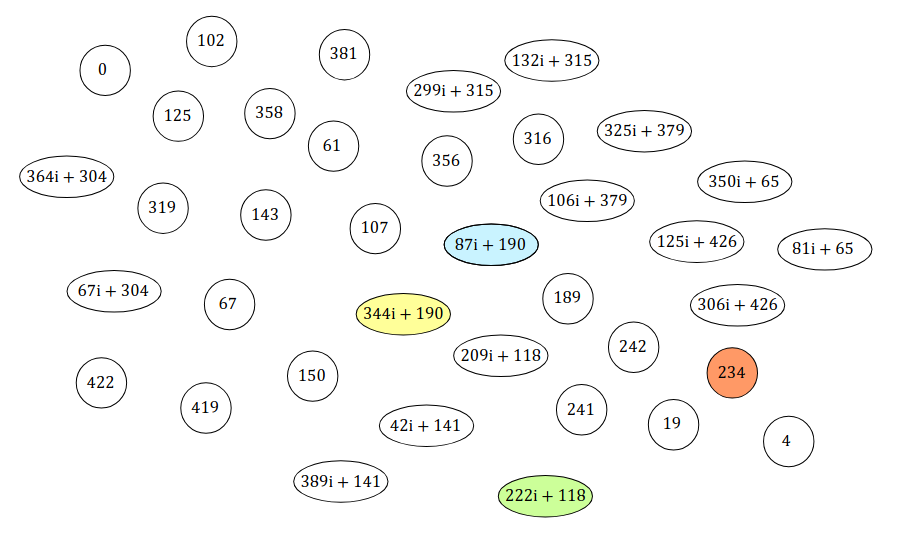
\includegraphics[width=0.7\textwidth]{isogenies}
	\caption{Пример графа для $p=431$}
	\label{fig:isogenies}
\end{figure}

Операции каждого из агентов создают различный набор дуг, которые соединяют узлы графа $j$-инвариантов. Они изображены на Рисунках \ref{fig:isogenies_a} и \ref{fig:isogenies_b}.

\begin{figure}[ht]
	\centering
	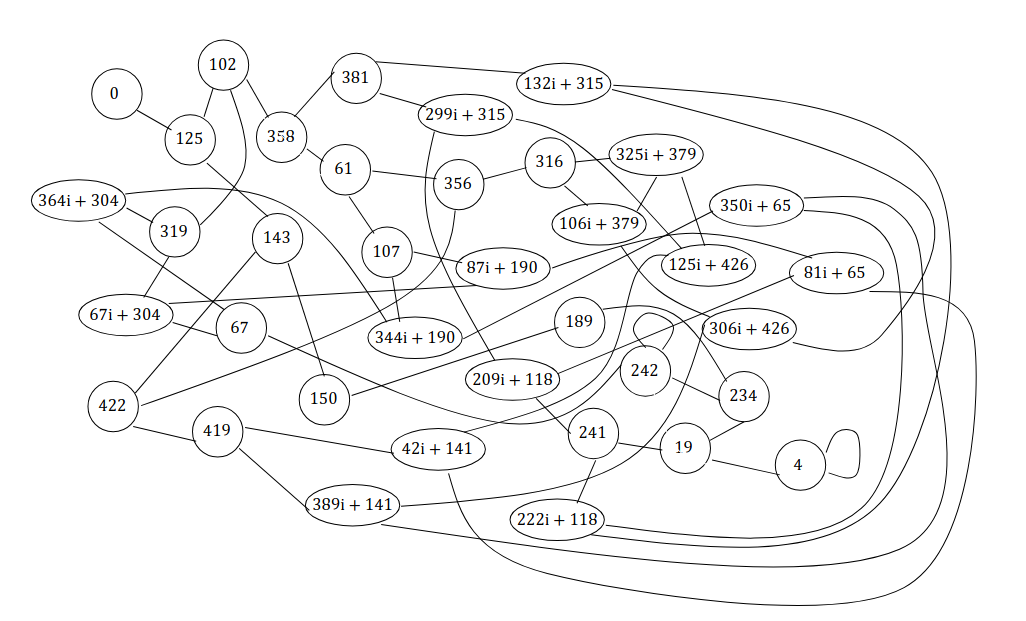
\includegraphics[width=0.7\textwidth]{isogenies_a}
	\caption{Граф агента А, связанный изогениями второго порядка (по три ребра из каждой вершины)}
	\label{fig:isogenies_a}
\end{figure}

\begin{figure}[ht]
	\centering
	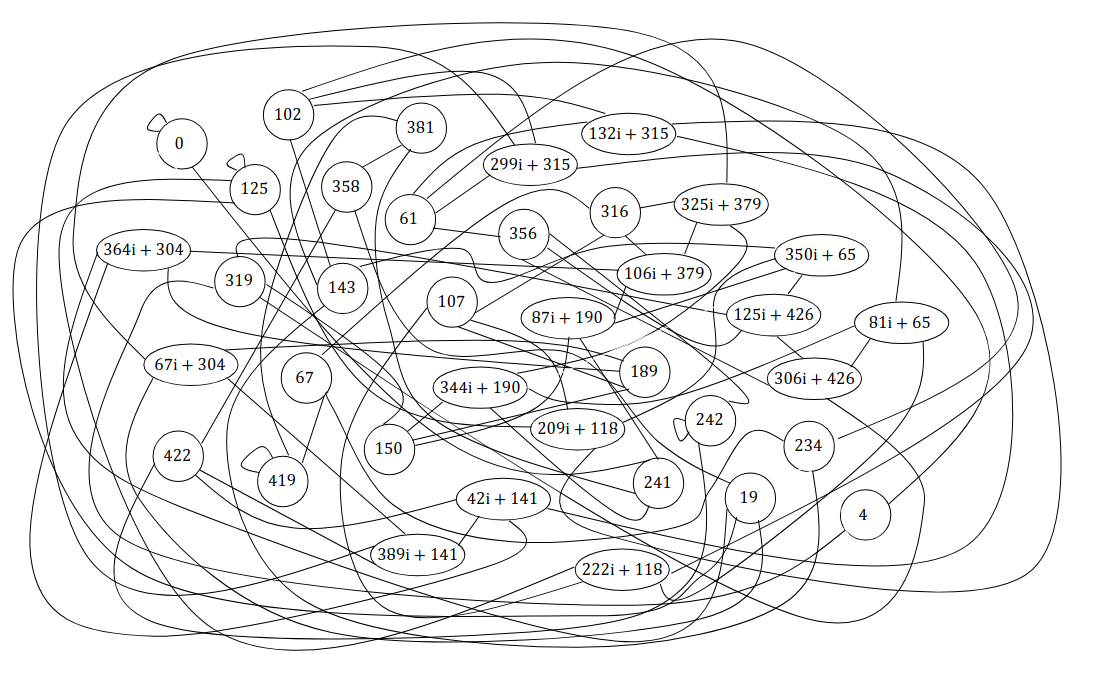
\includegraphics[width=0.7\textwidth]{isogenies_b}
	\caption{Граф агента Б, связанный изогениями третьего порядка (по четыре ребра из каждой вершины)}
	\label{fig:isogenies_b}
\end{figure}

Важно отметить, что для любого $p$ как бы мы не переставляли узлы, схема связей останется сложной. Это свойство отображает возможность добраться от одного узла до другого за малое число шагов.

Еще одним важным свойством является независимость полученных графов двух агентов.

Простое число $p$ выбирается особым образом:
\begin{equation*}
	p = 2^k 3^m - 1.
\end{equation*}
При этом числа $k$ и $m$ задают количество изогений (шагов в графе), которые совершат агенты А и Б, соответственно.

\section{Движение до открытого ключа}

В качестве начальных условий выступает $E_a$ -- некоторая эллиптическая кривая, задающая начальный $j$-инвариант.

Рассмотрим движение агента А по графу. Он выбирает точку $S$ порядка $\deg S = 2^4 = 16$.

На первом шаге он выполняет следующую последовательность операций:
\begin{equation*}
	S \rightarrow [2]S \rightarrow [4]S \rightarrow [8]S
\end{equation*}
\begin{equation*}
	\varphi_0: \ker \varphi_0 = \{ \mathcal{O}, [8]S \}.
\end{equation*}
Так он получает изогению $\varphi_0$ для перехода в другой узел.

Второй шаг:
\begin{equation*}
	S \rightarrow \varphi_0(S) \rightarrow [2] \varphi_0(S) \rightarrow [4] \varphi_0(S)
\end{equation*}
\begin{equation*}
	\varphi_0: \ker \varphi_1 = \{ \mathcal{O}, [4]\varphi_0(S) \}.
\end{equation*}
Так он получает следующую изогению $\varphi_1$ для перехода.

\begin{figure}[ht]
	\centering
	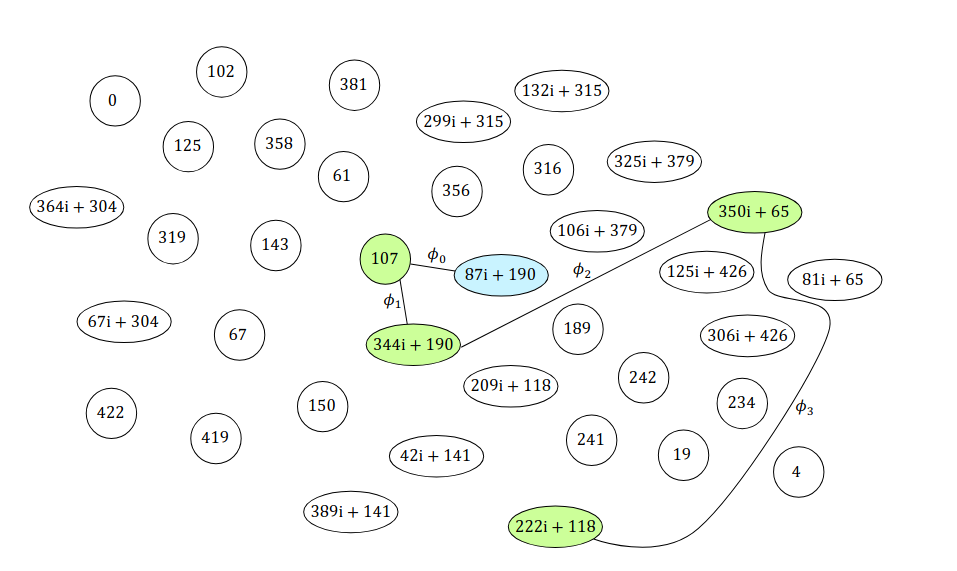
\includegraphics[width=0.7\textwidth]{steps_a}
	\caption{Шаги агента А}
	\label{fig:steps_a}
\end{figure}

Третий шаг:
\begin{equation*}
	S \rightarrow \varphi_0(S) \rightarrow \varphi_1(\varphi_0(S)) \rightarrow [2] \varphi_1(\varphi_0(S))
\end{equation*}
\begin{equation*}
	\varphi_2: \ker \varphi_2 = \{ \mathcal{O}, [2]\varphi_1(\varphi_0(S)) \}.
\end{equation*}

Четвертый шаг:
\begin{equation*}
	S \rightarrow \varphi_0(S) \rightarrow \varphi_1(\varphi_0(S)) \rightarrow \varphi_2(\varphi_1(\varphi_0(S)))
\end{equation*}
\begin{equation*}
	\varphi_3: \ker \varphi_3 = \{ \mathcal{O}, \varphi_2(\varphi_1(\varphi_0(S))) \}.
\end{equation*}

Агент Б проводит аналогично 3 шага с $\deg S = 27$, $[3]$ и $deg \varphi_i = 3$.

\begin{figure}[ht]
	\centering
	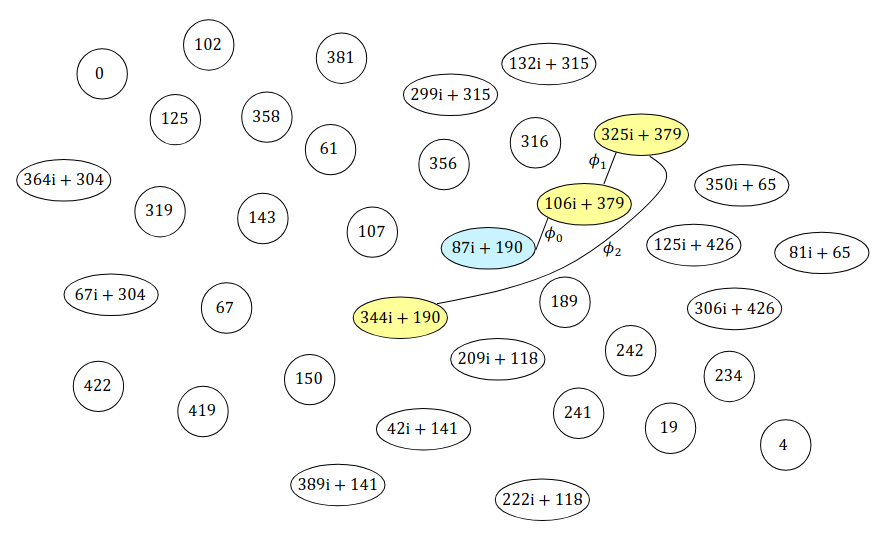
\includegraphics[width=0.7\textwidth]{steps_b}
	\caption{Шаги агента Б}
	\label{fig:steps_b}
\end{figure}

По итогу каждый из агентов получает $\{ S, \varphi_0, ... \varphi_m \}$ -- закрытый ключ, а также итоговый узел $E_n$ -- открытый ключ.

\section{Движение до общего секретного ключа}

Агенты А и Б передают друг другу их открытые ключи -- новые начальные узлы в графе. Они проводят точно такое же движение по графу, но уже с новых узлов.

\begin{figure}[ht]
	\centering
	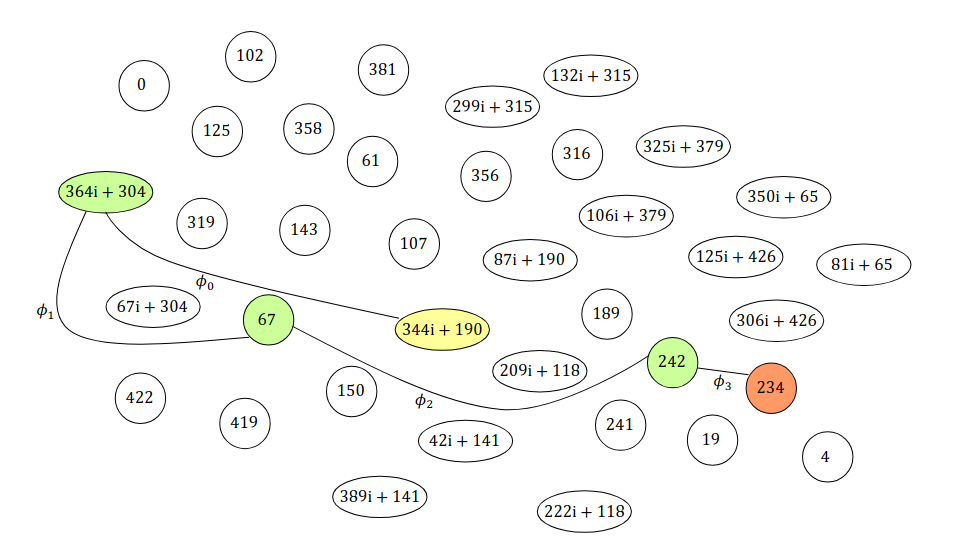
\includegraphics[width=0.7\textwidth]{secret_a}
	\caption{Шаги агента А}
	\label{fig:secret_a}
\end{figure}

\begin{figure}[ht]
	\centering
	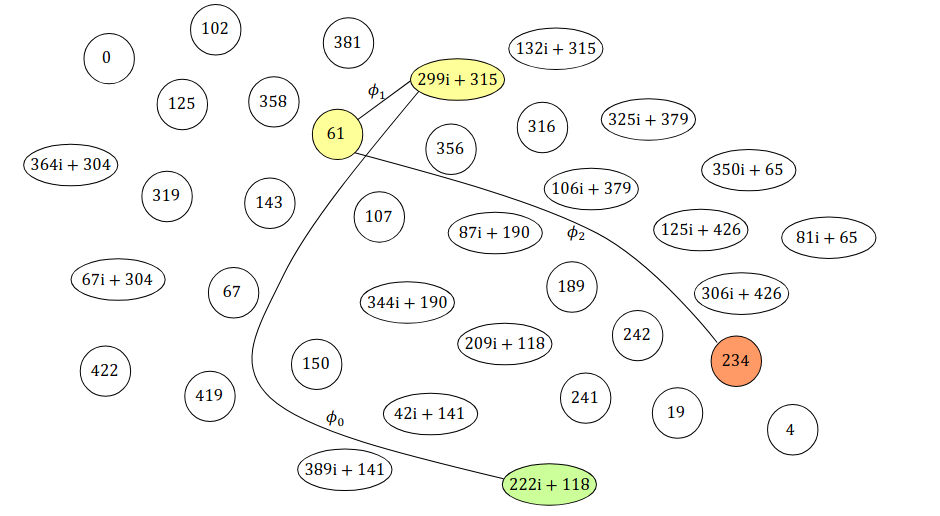
\includegraphics[width=0.7\textwidth]{secret_b}
	\caption{Шаги агента Б}
	\label{fig:secret_b}
\end{figure}

Все эти построения приводят А и Б к общему узлу. При этом злоумышленник имеет лишь начальный узел и два открытых ключа. Изогении, приводящие к этому ключу, получены как композиция большого количества изогений малого порядка. Они имеют очень высокую степень, а сложность поиска обратного пути экспоненциально растет с порядком изогении \cite{isogenies}.

\endinput
                                     % Вторая глава
\chapter{Заключение}

Приход квантовых компьютеров угрожает большому количеству используемых алгоритмов, поэтому конфиденциальность информации фундаментально зависит от развития постквантового шифрования .
Более того, оно стимулирует развитие криптографии в целом, повышая актуальность исследования как квантовых, так и неквантовых алгоритмов шифрования и взлома.

К счастью, этой области уделяется все больше внимания как со стороны государственных структур \cite{nsa_pqc}, так и частных компаний \cite{nvidia_pqc}. Например, NIST проводит отбор и стандартизацию алгоритмов постквантового шифрования. В процессе отбора были найдены важные уязвимости, в том числе в последнем раунде был взломан вышеописанный алгоритм SIDH, причем неквантовым алгоритмом \cite{sidh_broken}. Более тщательное изучение уже используемых алгоритмов (например, McEliece) повышает уверенность в том, что они действительно надежны в том числе против классических атак.

Задачи, лежащие в основе шифрования, опираются на новые, сложные абстракции. Использование этих задач в шифровании, поиск уязвимостей в алгоритмах приводит к более глубоким математическим исследованиям, развивая математическую область, на которую опирается шифрование.

Таким образом, потенциальное появление квантовых компьютеров повысило внимание, уделяемое безопасности информации, а оно, в свою очередь, дало толчок к развитию математических и криптографических направлений.

\endinput                                     % Третья глава

\printbibliography[title=Список использованных источников] % Автособираемый список литературы

\end{document}